\documentclass[11pt]{beamer}
\usetheme{CambridgeUS}

\usepackage[utf8]{inputenc}
\usepackage[english]{babel}
\usepackage{amsmath}
\usepackage{amsfonts}
\usepackage{amssymb}
\usepackage{graphicx}

\author{Jonathan Sidi}
\title[Election Analysis]{Real Time Tracking and Analysis of Election Polling in Israel}
%\subtitle{}
%\logo{}
\institute[Hebrew University]{Department of Statistics, Hebrew University of Jerusalem}
\date{May 28, 2015}
%\subject{}
%\setbeamercovered{transparent}
%\setbeamertemplate{navigation symbols}{}

\begin{document}
\maketitle

\begin{frame}
\begin{block}{An open source web application which gathers continuously updated polling information to one interactive location}
\end{block}

\begin{itemize}
\item Stay Up to Date
\item Interactive Plotting with Raw Data
\item Party Mandate Simulator
\item User Generated Coalitions
\end{itemize}
\end{frame}

\section{Quickview}
\begin{frame}{Up to Date Polls}
				\begin{figure}[h]
				\centering
				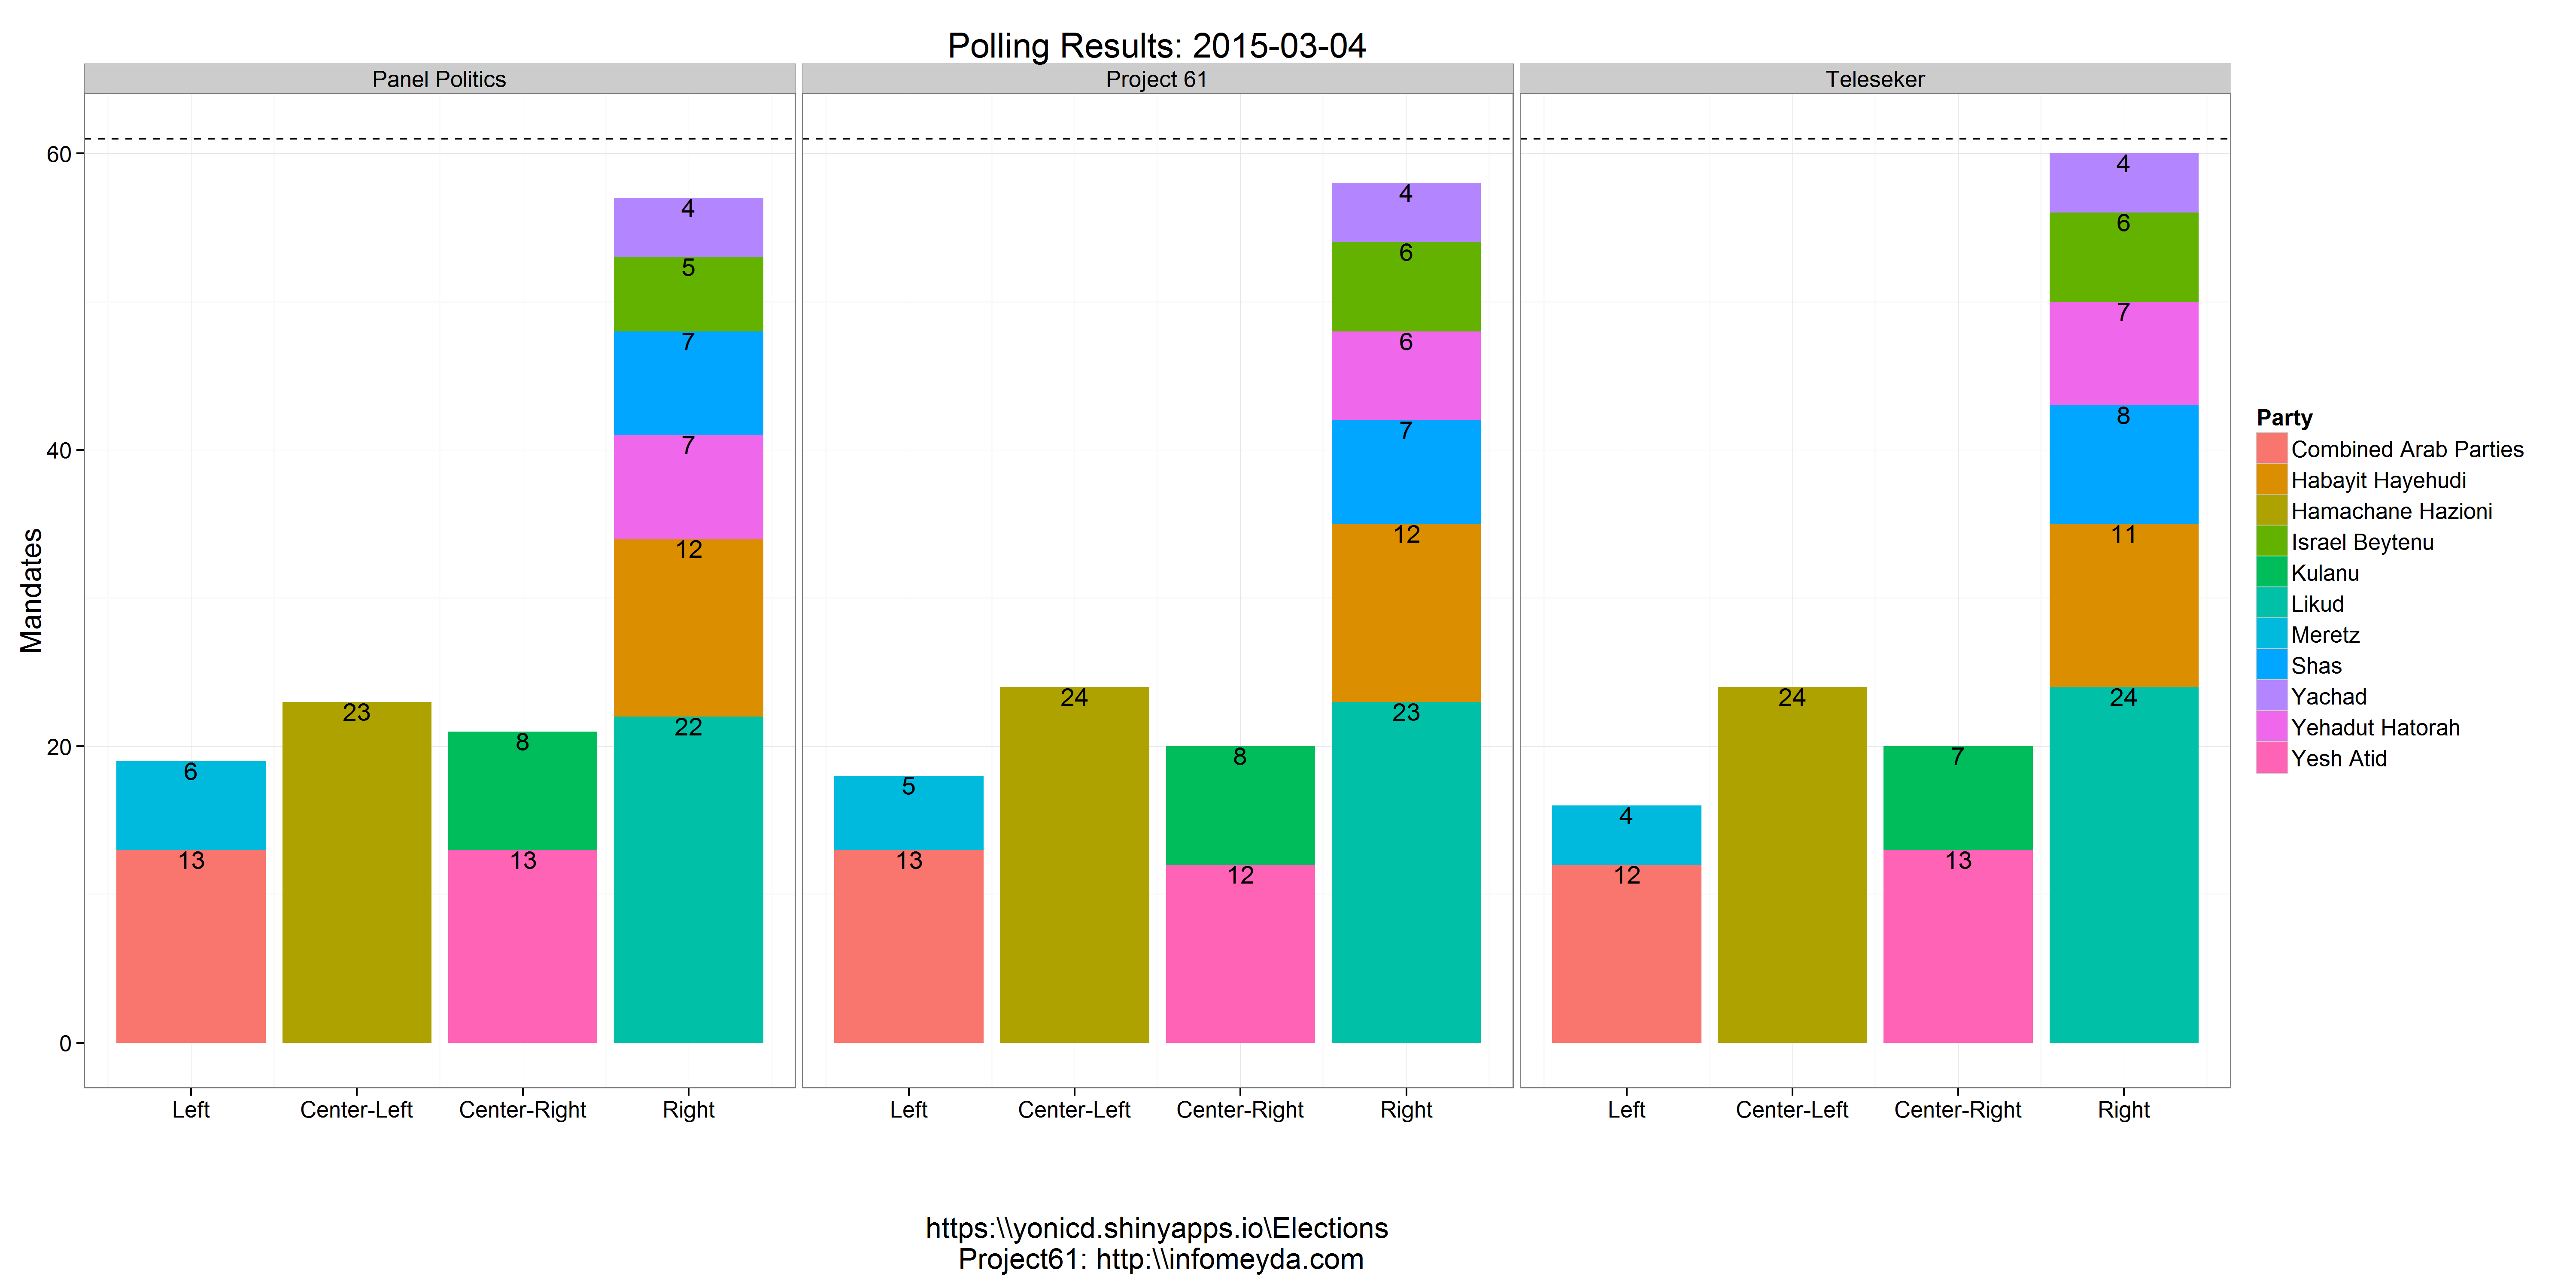
\includegraphics[width=1\linewidth]{../www/LastDayPlot}
				\label{fig:LastDayPlot}
				\end{figure}
\begin{block}{Stay up to date with latest polling results from all the pollsters}
\end{block}
\end{frame}

\section{Interactive}
\begin{frame}{Interactive Graphs}
				\begin{figure}[h]
					\centering
					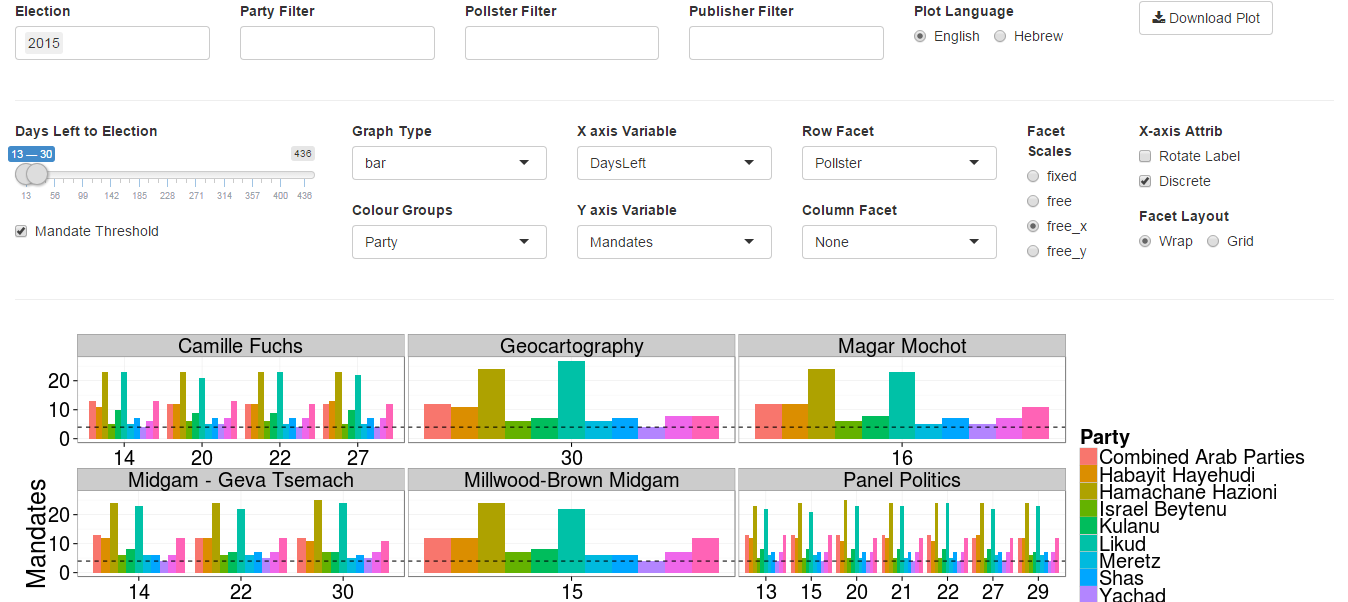
\includegraphics[width=1\linewidth]{../www/pad_screen_grab}
					\label{fig:pad_screen_grab}
				\end{figure}
\begin{block}{Freedom to choose dimensions and layout of the data to view}
\end{block}
\end{frame}

\begin{frame}{Example: Cross Section Analysis}
				\begin{figure}[h]
					\centering
					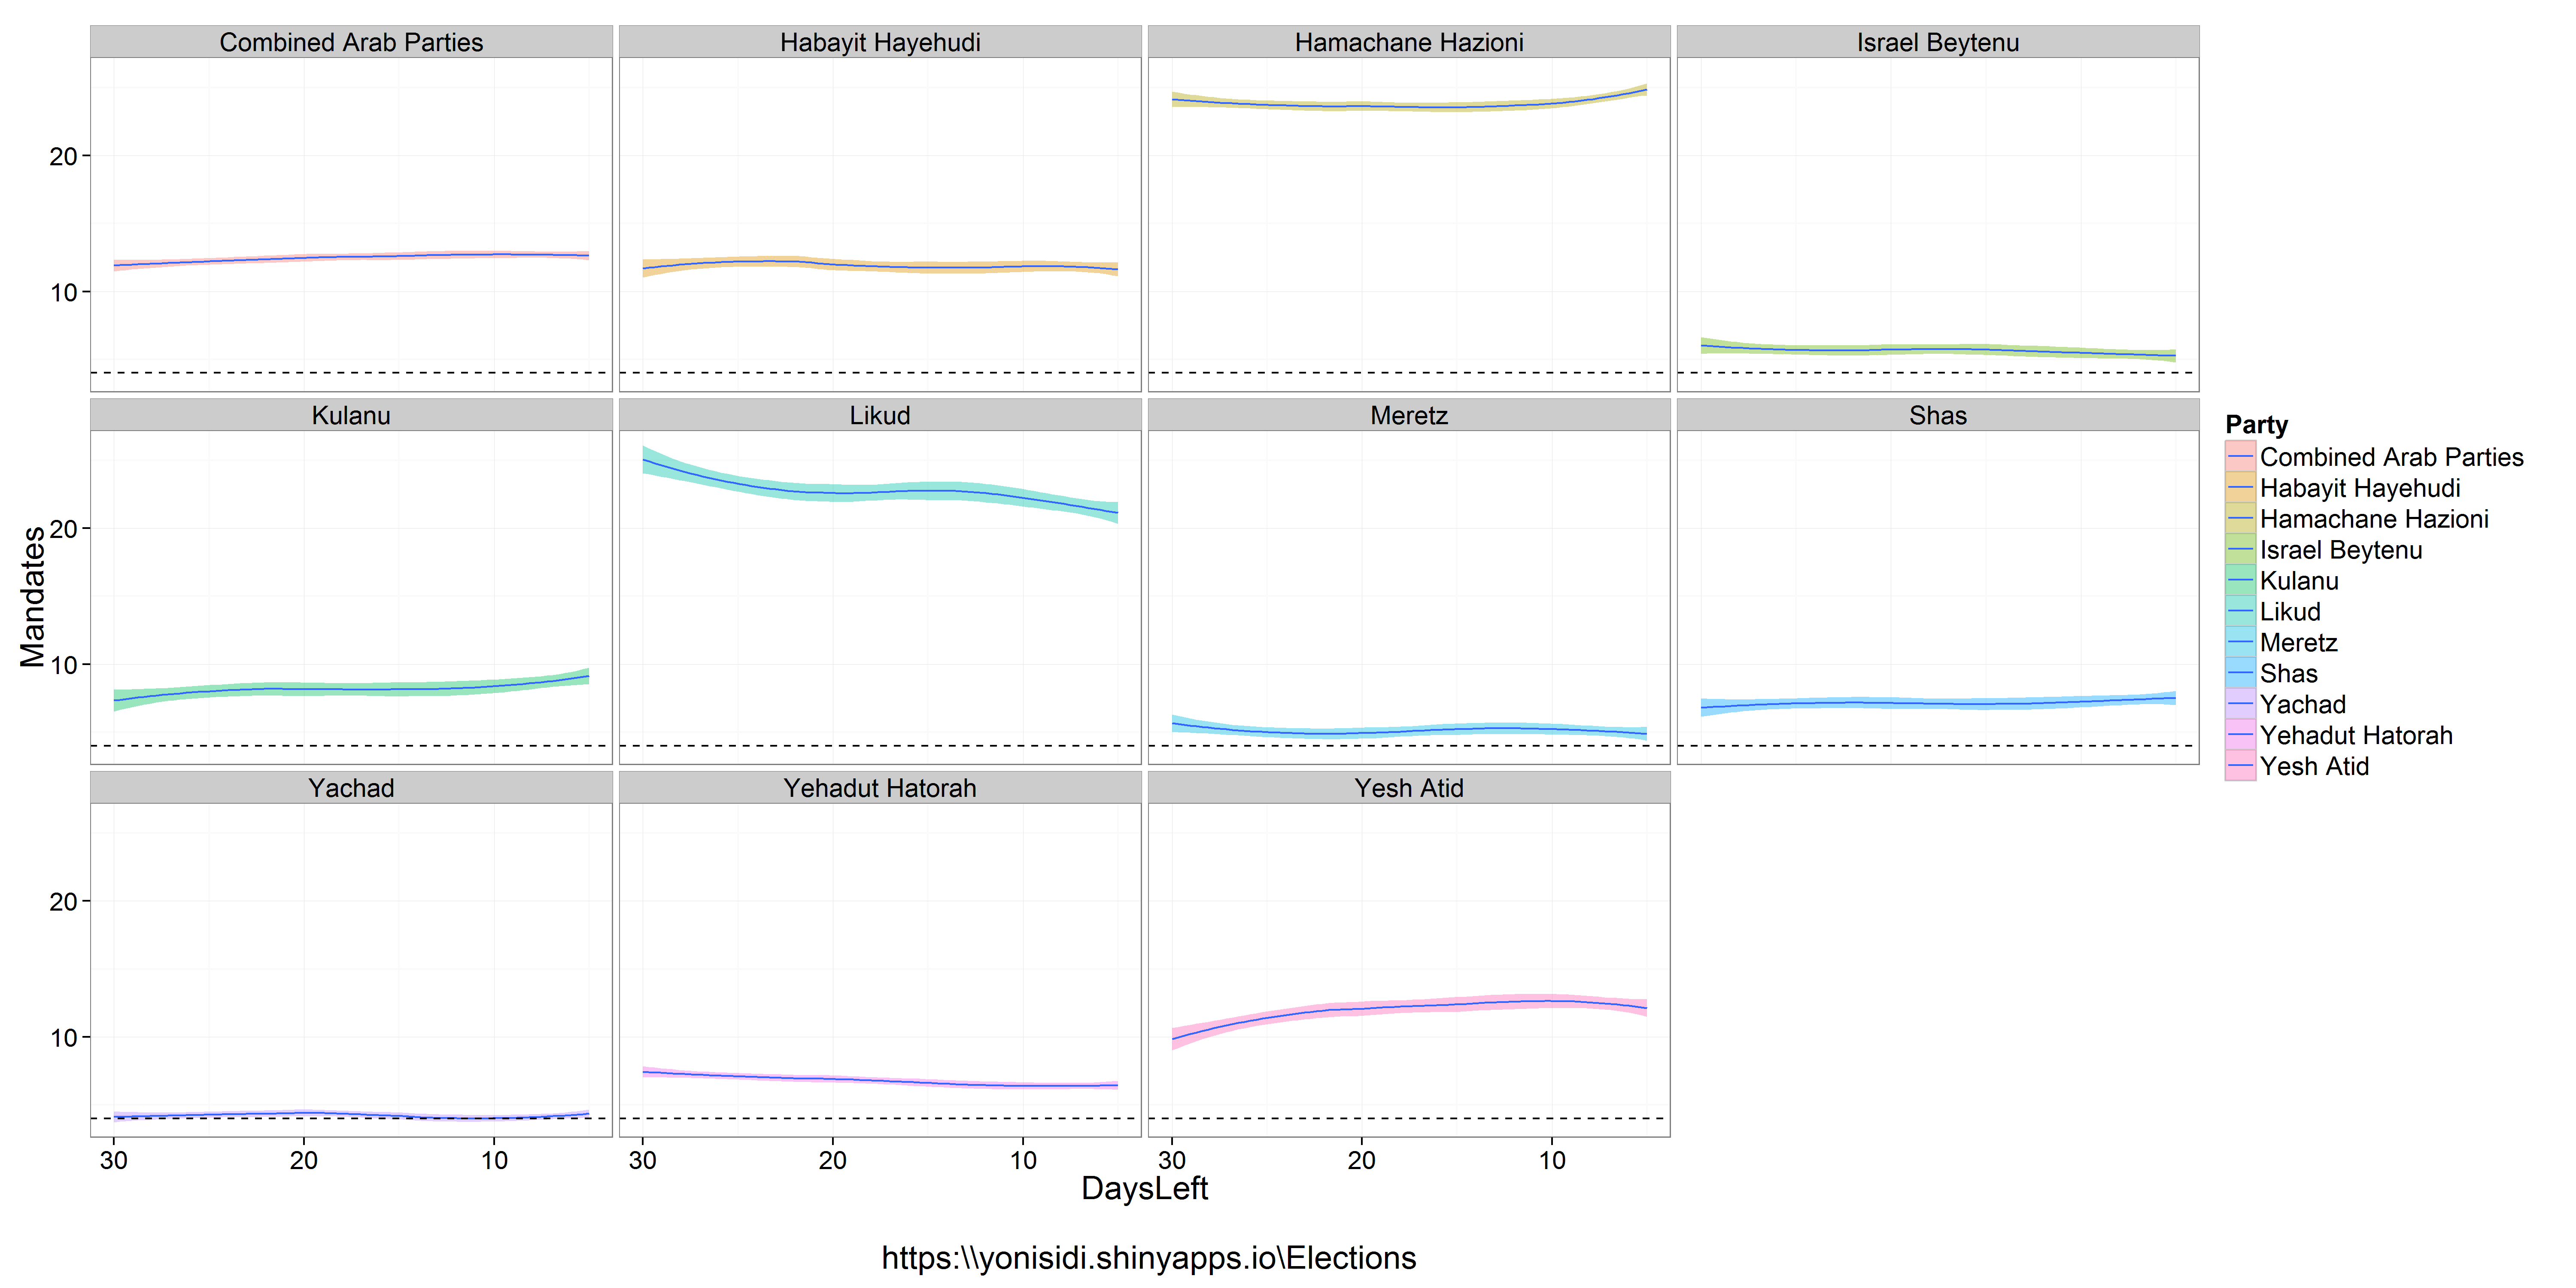
\includegraphics[width=1\linewidth]{../www/ElectionPlot_trend}
					\label{fig:ElectionPlot_trend}
				\end{figure}
\begin{block}{Comparison of pollster results within parties to find public sentiment variablilty and pollster estimation bias}
\end{block}				
\end{frame}				

\begin{frame}{Example: Longitudintal Analysis}				
				\begin{figure}[h]
					\centering
					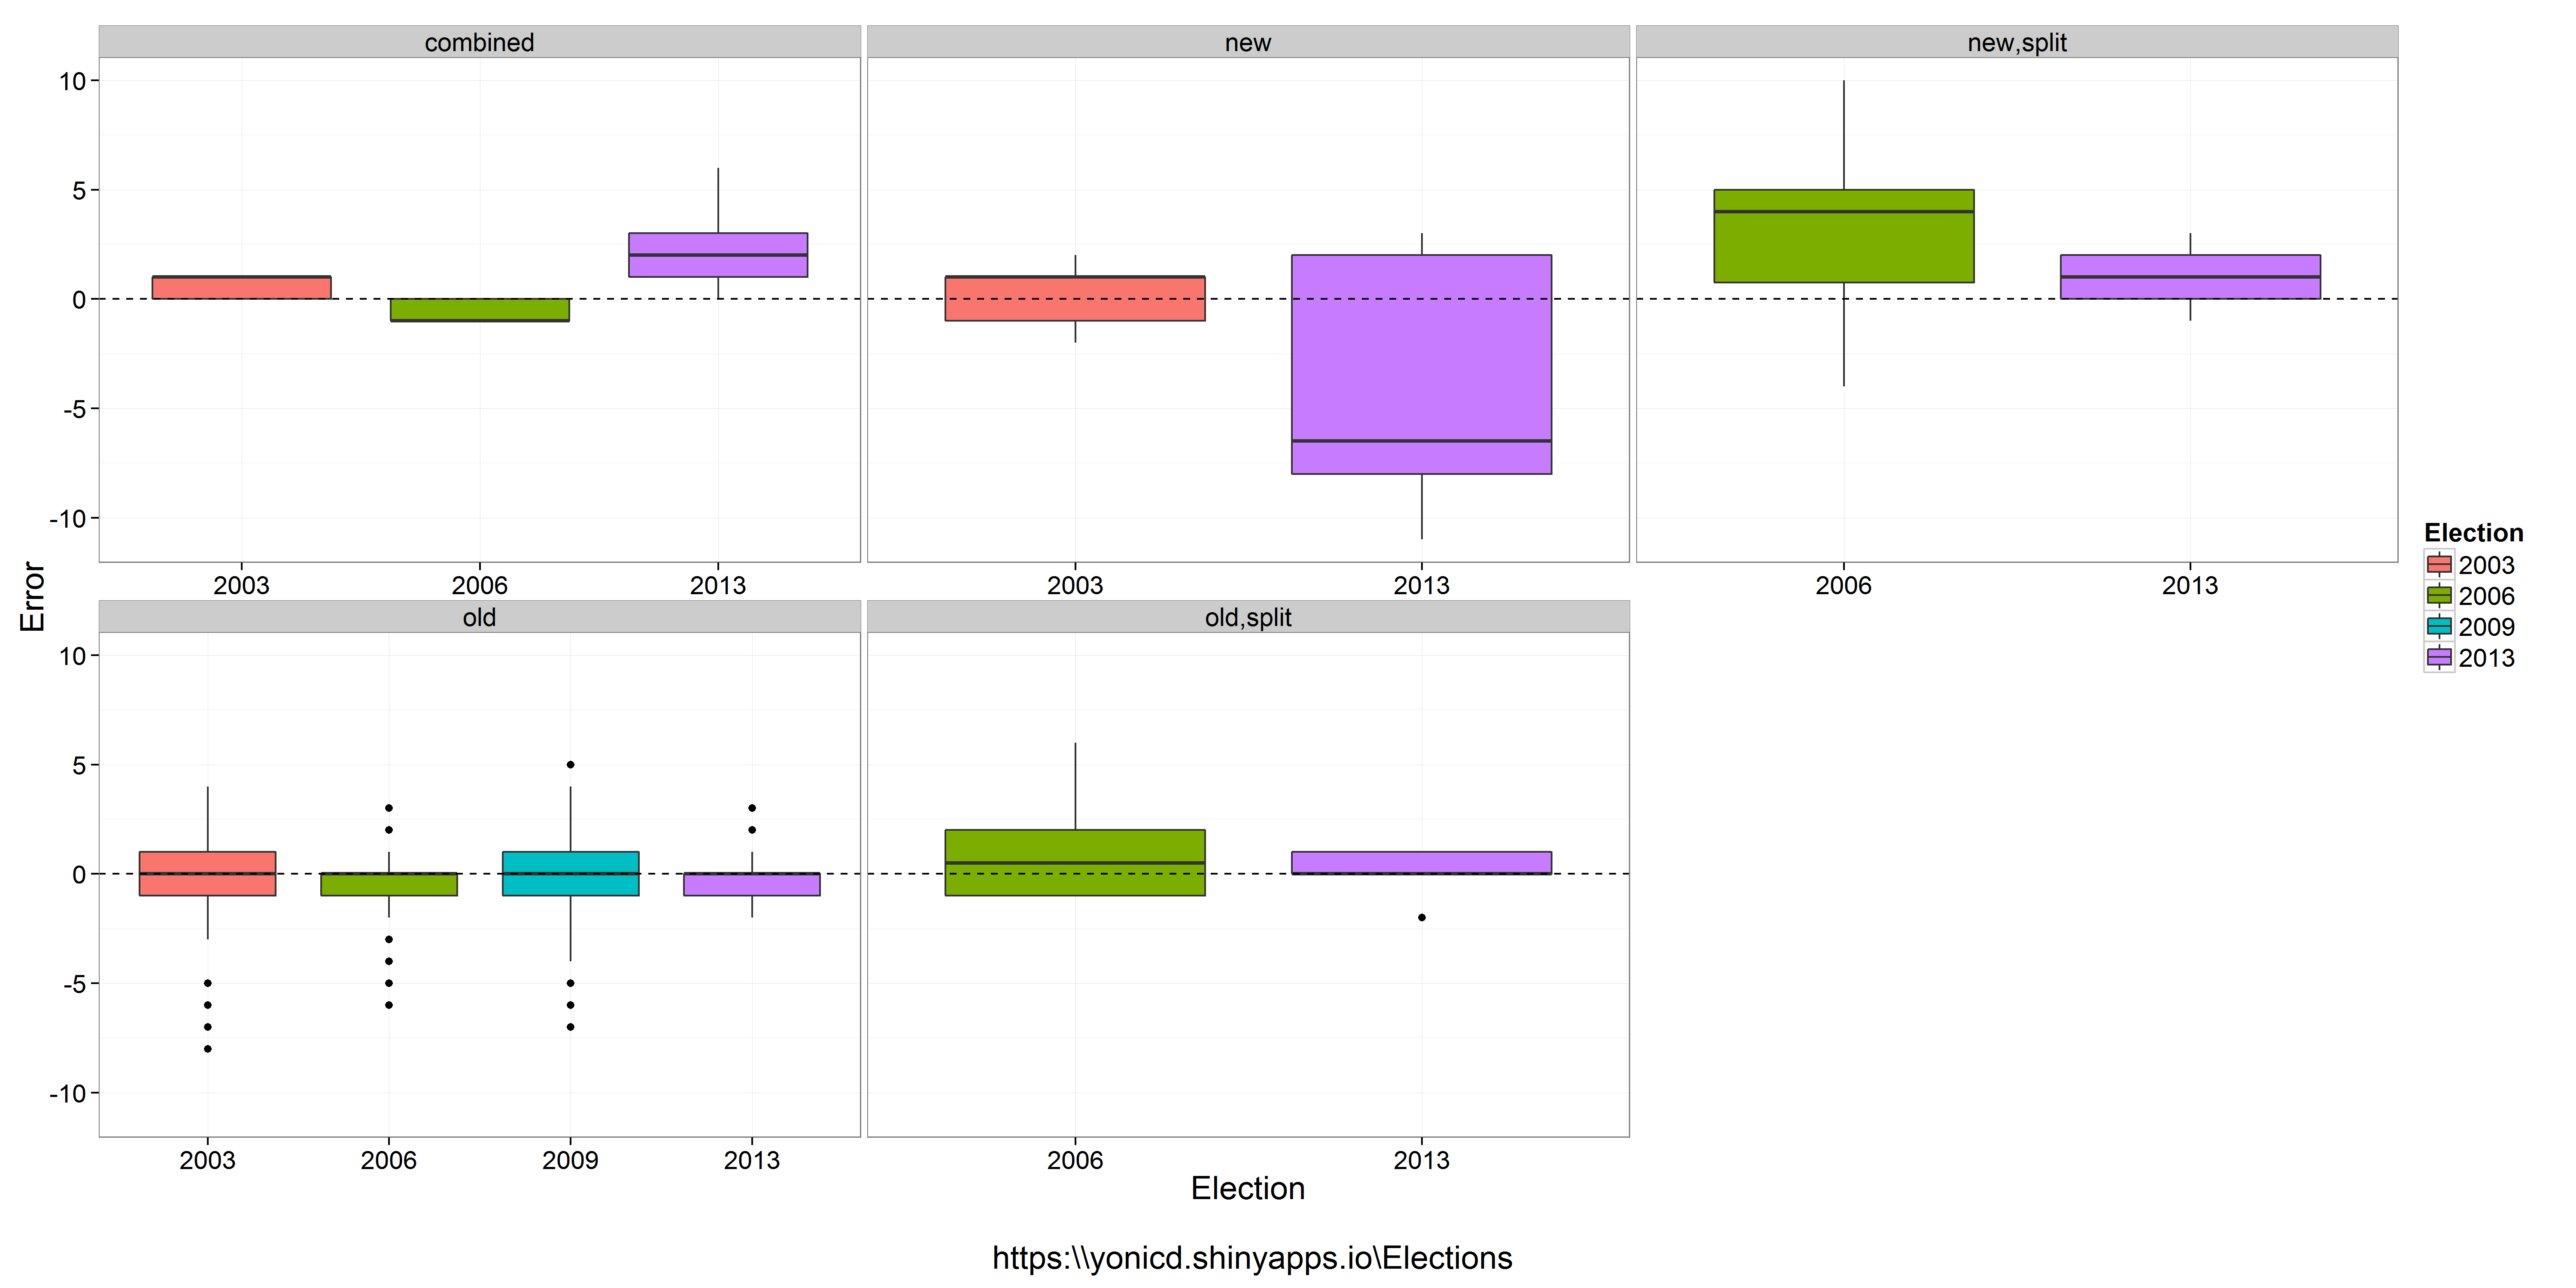
\includegraphics[width=1\linewidth]{../www/ElectionPlot_longitudinal}					\label{fig:ElectionPlot_longitudinal}
				\end{figure}
\begin{block}{Compare party outcomes or pollster errors across elections}\end{block}
\end{frame}

\section{Simulator}
\begin{frame}{Mandate Simulator}
\begin{figure}				
					\centering
					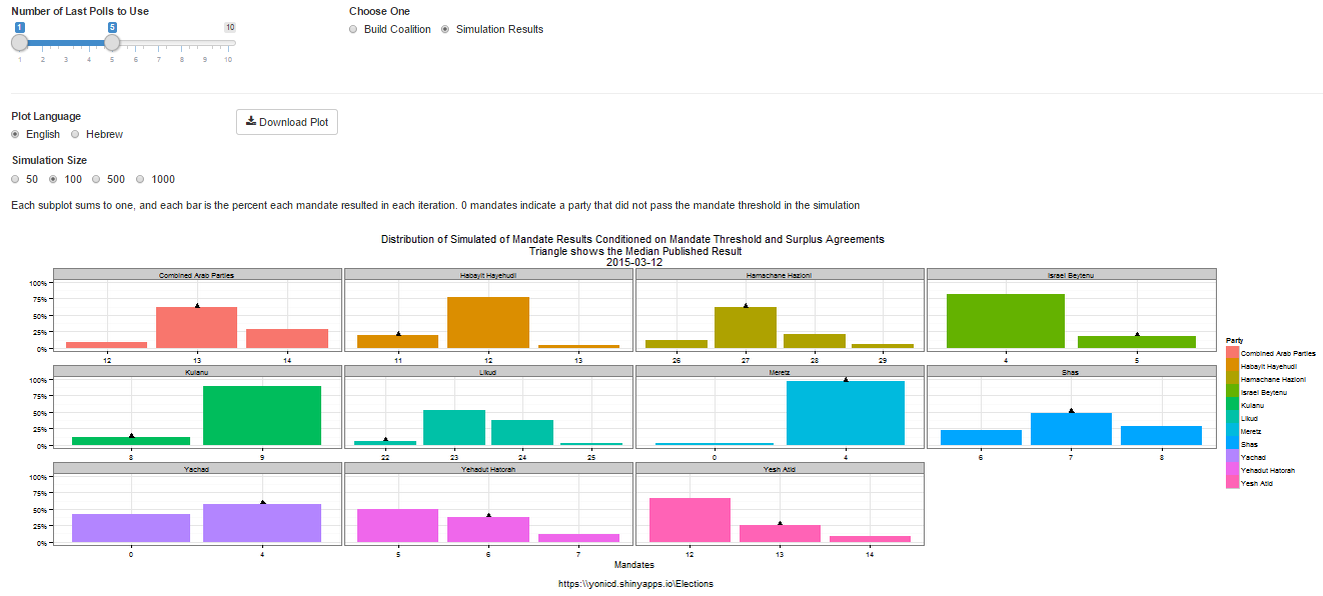
\includegraphics[width=1\linewidth]{../www/sim_screen_grab}
					\label{fig:sim_screen_grab}
				\end{figure}
			\begin{block}{Bootstrap simulation is performed using the published sampling error to reproduce the distribution of mandates for each party.}
			\end{block}
\end{frame}


\section{User Generated Coalitions}
\begin{frame}{Coalition White board}

	\begin{figure}[h]
					\centering
					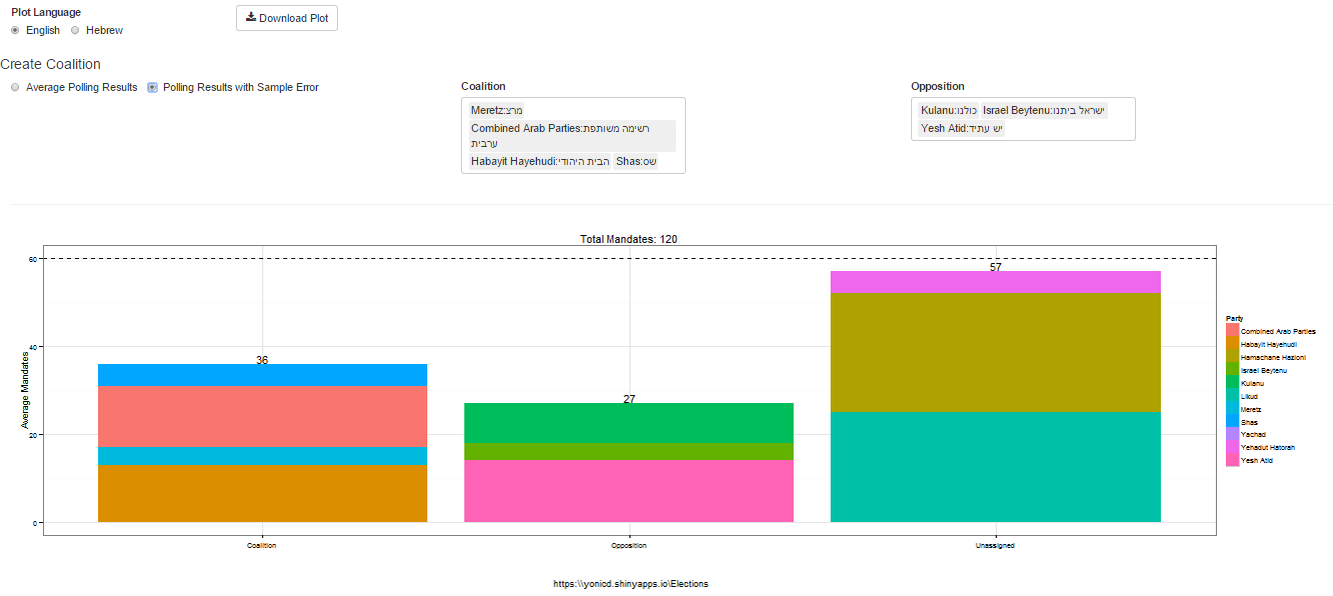
\includegraphics[width=1\linewidth]{../www/coal_screen_grab}
					\label{fig:coal_screen_grab}
	\end{figure}
\begin{block}{Create coalitions based on either the simulated distribution or actual published polls and see who can pass 60 mandates}
\end{block}
\end{frame}

\end{document}